% !TEX program = xelatex
% =============================================================================
% Pixel Round — Lesson Plan (en-US)
% Adapted for a U.S. public high school senior class (12th grade)
% Visual identity mirrors docs_math/Pixel_Round_Math_en-US.pdf
% Compile:  xelatex Plano_de_Aula_en-US.tex   (run twice for TOC + refs)
% =============================================================================
\documentclass[12pt,letterpaper]{scrartcl}

% ---------- Language & fonts -------------------------------------------------
\usepackage{fontspec}
\usepackage{polyglossia}
\setdefaultlanguage{english}
\PolyglossiaSetup{english}{indentfirst=false}
\setmainfont{Latin Modern Roman}[Scale=1.08]
\setsansfont{Latin Modern Sans}[Scale=1.08]
\setmonofont{Latin Modern Mono}[Scale=1.00]
\usepackage{unicode-math}
\setmathfont{Latin Modern Math}[Scale=1.08]

% ---------- Packages ---------------------------------------------------------
\usepackage{amsmath}
\usepackage{mathtools}

\usepackage[letterpaper,top=1in,bottom=1in,left=1in,right=1in,
            headheight=16pt]{geometry}
\usepackage{microtype}
\usepackage{xcolor}
\usepackage{booktabs}
\usepackage{array}
\usepackage{tabularx}
\usepackage{enumitem}
\usepackage{titlesec}
\usepackage{fancyhdr}
\usepackage{graphicx}
\usepackage{csquotes}
\usepackage{tcolorbox}
\tcbuselibrary{skins,breakable}
\usepackage{needspace}                   % evita orfas em caixas didaticas
\usepackage{caption}
\usepackage{subcaption}
\usepackage{float}                       % [H] = "exatamente aqui, sem float"

\raggedbottom                            % paginas terminam onde o texto termina
\usepackage[colorlinks=true,
            linkcolor=linkc,
            urlcolor=linkc,
            citecolor=linkc,
            bookmarks=true,bookmarksopen=true,
            pdftitle={Pixel Round — Lesson Plan (en-US)},
            pdfauthor={Vinícius Rodrigues de Souza}]{hyperref}

% ---------- Color palette (project canonical) --------------------------------
\definecolor{accent}{HTML}{CC2020}
\definecolor{ink}{HTML}{1F1F23}
\definecolor{muted}{HTML}{4E4E58}
\definecolor{bg}{HTML}{FBF6E9}
\definecolor{rule}{HTML}{D8D1BC}
\definecolor{linkc}{HTML}{8A0F0F}             % links: tom mais escuro do accent

\color{ink}

% Penalidades altas contra orfas / viuvas globalmente
\widowpenalty=10000
\clubpenalty=10000

% ---------- Section styling --------------------------------------------------
\titleformat{\section}
  {\sffamily\Large\bfseries\color{accent}}{\thesection.}{0.6em}{}
\titleformat{\subsection}
  {\sffamily\large\bfseries\color{accent!85!ink}}{\thesubsection}{0.6em}{}
\titleformat{\subsubsection}
  {\sffamily\normalsize\bfseries\color{muted}}{\thesubsubsection}{0.5em}{}
\titlespacing*{\section}{0pt}{1.2\baselineskip}{0.6\baselineskip}
\titlespacing*{\subsection}{0pt}{0.8\baselineskip}{0.3\baselineskip}
\titlespacing*{\subsubsection}{0pt}{0.6\baselineskip}{0.2\baselineskip}

% ---------- Headers & footers ------------------------------------------------
\pagestyle{fancy}
\fancyhf{}
\fancyhead[L]{\small\sffamily\bfseries\color{accent}PIXEL ROUND}
\fancyhead[R]{\small\sffamily\color{muted}Lesson Plan --- Grade 12}
\fancyfoot[L]{\small\sffamily\color{muted}Pixel Round --- Teacher resource}
\fancyfoot[R]{\small\sffamily\color{muted}Page \thepage}
\renewcommand{\headrulewidth}{0.4pt}
\renewcommand{\footrulewidth}{0.4pt}
\renewcommand{\headrule}{{\color{rule}\hrule height \headrulewidth}}
\renewcommand{\footrule}{{\color{rule}\vskip-\footrulewidth\hrule height \footrulewidth\vskip-\footrulewidth}}

% ---------- Didactic boxes ---------------------------------------------------
\newtcolorbox{formula}{
  colback=bg, colframe=rule, boxrule=0.4pt, arc=2pt,
  left=10pt,right=10pt,top=8pt,bottom=8pt,
  before skip=8pt, after skip=8pt,
  fontupper=\color{accent}, breakable,
  before={\par\needspace{4\baselineskip}}
}

\newtcolorbox{activity}[1][Activity]{
  enhanced, breakable,
  colback=bg, colframe=accent, boxrule=0.6pt, arc=4pt,
  left=12pt,right=12pt,top=10pt,bottom=10pt,
  before skip=12pt, after skip=12pt,
  before={\par\needspace{14\baselineskip}},
  attach boxed title to top left={xshift=10pt,yshift=-8pt},
  boxed title style={colback=accent,colframe=accent,boxrule=0pt,arc=2pt},
  coltitle=white, fonttitle=\sffamily\bfseries\small,
  title=#1
}

\newtcolorbox{note}[1][Teacher note]{
  enhanced, breakable,
  colback=bg!50!white, colframe=rule, boxrule=0.4pt, arc=2pt,
  left=10pt,right=10pt,top=8pt,bottom=8pt,
  before skip=8pt, after skip=8pt,
  before={\par\needspace{6\baselineskip}},
  attach boxed title to top left={xshift=10pt,yshift=-7pt},
  boxed title style={colback=muted,colframe=muted,boxrule=0pt,arc=2pt},
  coltitle=white, fonttitle=\sffamily\bfseries\footnotesize,
  title=#1
}

\newtcolorbox{standard}[1][Standard]{
  enhanced, breakable,
  colback=bg!70!white, colframe=accent!60!ink, boxrule=0.4pt, arc=2pt,
  left=10pt,right=10pt,top=6pt,bottom=6pt,
  before skip=6pt, after skip=6pt,
  before={\par\needspace{4\baselineskip}},
  attach boxed title to top left={xshift=10pt,yshift=-6pt},
  boxed title style={colback=accent!60!ink,colframe=accent!60!ink,boxrule=0pt,arc=2pt},
  coltitle=white, fonttitle=\sffamily\bfseries\footnotesize,
  title=#1
}

\setlength{\parskip}{0.75em}
\setlength{\parindent}{0pt}
\linespread{1.10}

\newcommand{\code}[1]{\texttt{\small #1}}
\newcommand{\acc}[1]{\textcolor{accent}{\textbf{#1}}}
\newcommand{\timing}[1]{\textnormal{\footnotesize\color{bg!90!white}\textsf{#1}}}

% Configuracao de legendas
\captionsetup{font=small, labelfont={bf,color=accent}, textfont={color=muted}, justification=centering}
\captionsetup[sub]{font=footnotesize, labelfont={bf,color=accent!75!ink}, textfont={color=muted}}

% Espacamento das figuras
\setlength{\textfloatsep}{14pt plus 2pt minus 2pt}
\setlength{\floatsep}{14pt plus 2pt minus 2pt}
\setlength{\intextsep}{14pt plus 2pt minus 2pt}

\graphicspath{{img/}}

\begin{document}

% =============================================================================
% COVER
% =============================================================================
\begin{titlepage}
  \centering
  \vspace*{3.2cm}
  {\sffamily\bfseries\fontsize{56}{60}\selectfont \color{accent} Pixel Round\par}
  \vspace{0.7cm}
  {\sffamily\LARGE\color{muted} Lesson Plan\par}
  \vspace{0.25cm}
  {\sffamily\Large\color{muted} Grade 12 --- High School Senior Year\par}
  \vspace{1.4cm}
  {\color{rule}\rule{0.6\textwidth}{0.6pt}\par}
  \vspace{0.9cm}
  \begin{minipage}{0.84\textwidth}
    \centering\color{ink}\large
    A four-period instructional sequence that uses the open
    \emph{Pixel Round} generator to ground senior-year geometry
    in a problem that students can both see and code: how to
    represent a continuous curve on a finite grid of pixels.
    Designed for U.S. public high schools, aligned to the Common
    Core State Standards.
  \end{minipage}
  \vspace{0.9cm}\\
    \vspace{1.4cm}
  \begin{minipage}{0.78\textwidth}
    \centering
    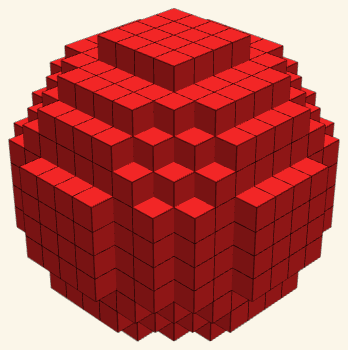
\includegraphics[width=0.55\linewidth]{fig07_3d_sphere_d12.png}\\[0.6em]
    {\sffamily\footnotesize\color{muted}Voxelised sphere of diameter 12 generated by Pixel Round.}
  \end{minipage}
  \vspace{1.0cm}\\
  {\color{rule}\rule{0.6\textwidth}{0.6pt}\par}
  \vspace{1.0cm}
{\color{rule}\rule{0.6\textwidth}{0.6pt}\par}
  \vspace{1.8cm}
  \begin{minipage}{0.82\textwidth}
    \centering\sffamily\small\color{muted}
    \textbf{Cross-curricular:} Mathematics $\cdot$ Computer Science $\cdot$ Visual Art $\cdot$ Physics \\[0.4em]
    \textbf{Alignment:} Common Core State Standards $\cdot$ NCTM Principles to Actions $\cdot$ CAST Universal Design for Learning
  \end{minipage}
\end{titlepage}

% =============================================================================
% TOC
% =============================================================================
\renewcommand{\contentsname}{\color{accent}Contents}
\tableofcontents
\thispagestyle{fancy}
\newpage

% =============================================================================
\section{Overview at a glance}

\begin{center}
\begin{tabular}{@{}p{0.30\textwidth}p{0.64\textwidth}@{}}
\toprule
\textbf{Subject} & Mathematics (Geometry, Algebra II, or Pre-Calculus strand). \\
\addlinespace[2pt]
\textbf{Grade level} & 12 (high school senior year). Adaptable to grades 10--11. \\
\addlinespace[2pt]
\textbf{Setting} & Traditional brick-and-mortar public high school. Adaptations included for hybrid and remote delivery. \\
\addlinespace[2pt]
\textbf{Duration} & 4 class periods of 50 minutes (200 instructional minutes). Block-scheduling variant (2 periods of 90 minutes) outlined in §\ref{sec:adapt}. \\
\addlinespace[2pt]
\textbf{Core resource} & Pixel Round --- free, in-browser web app. No account, no installation, no data collection. Works offline as a PWA. \\
\addlinespace[2pt]
\textbf{Standards focus} & CCSS.MATH.CONTENT.HSG.GPE $\cdot$ HSG.GMD $\cdot$ Mathematical Practices MP4, MP5, MP7. \\
\addlinespace[2pt]
\textbf{Cross-curricular} & AP Computer Science Principles $\cdot$ Visual Arts (digital media) $\cdot$ Physics (waves and acoustics). \\
\addlinespace[2pt]
\textbf{Student prerequisites} & Coordinate plane, equation of a circle, area/volume of basic solids, function notation, percent and ratio. \\
\addlinespace[2pt]
\textbf{Teacher prep} & 15 min in Pixel Round; skim \texttt{docs\_math/Pixel\_Round\_Math\_en-US.pdf} for the math underneath. \\
\bottomrule
\end{tabular}
\end{center}

\begin{note}[Equity and access]
This plan was deliberately designed around U.S. public-school realities: 1:1 Chromebook fleets, district web filters, mixed device readiness, students with IEPs and 504 plans, and English Learners at varying proficiency levels. Pixel Round runs on any Chromebook manufactured in the last decade, requires no login, and is small enough that a single classroom Wi-Fi cache will serve it offline for the rest of the period. A fully \emph{analog} fallback (graph paper, no devices) is described in Appendix~\ref{ap:adapt}.
\end{note}

% =============================================================================
\section{Rationale and pedagogical grounding}

Pixel art and voxel art saturate the visual diet of an American teenager --- from Minecraft and Stardew Valley to the icon set on their phone. Treating that everyday aesthetic as a \emph{mathematical artifact} converts a familiar surface into an authentic problem: how does a computer, which can only fill rectangular cells, represent a curve defined on the continuum $\mathbb{R}$?

The lesson is built on the \acc{5E instructional model} (Bybee et al., 2006): \emph{Engage, Explore, Explain, Elaborate, Evaluate}. Each of the four class periods walks through all five phases in different proportions, ramping from concrete (drawing on graph paper) to abstract (the implicit equation of an ellipsoid) and back to applied (a student-authored composition with a math defense).

Three deeper commitments structure the sequence:

\begin{itemize}[leftmargin=1.3em,itemsep=0.15em,topsep=0.3em]
  \item \acc{Conceptual understanding over procedure} (NCTM, \emph{Principles to Actions}, 2014). The same continuous circle admits three different discrete renderings depending on which inclusion rule we pick. Students do not memorize three algorithms --- they discover that the choice matters.
  \item \acc{Use of appropriate tools strategically} (CCSS Mathematical Practice MP5). Pixel Round is not a calculator: it is a sandbox for testing mathematical hypotheses about which cells should be filled.
  \item \acc{Universal Design for Learning} (CAST UDL Guidelines, version 2.2). Every lesson offers \emph{multiple means of engagement} (game culture entry point, autonomy in the final project), \emph{multiple means of representation} (visual, algebraic, computational), and \emph{multiple means of action and expression} (drawing, computing, justifying in writing or orally).
\end{itemize}

\begin{note}[Why \emph{not} just teach the unit circle?]
The conventional Geometry unit on circles asks students to recall $x^2 + y^2 = r^2$ and apply it to ten short problems. Pixel Round inverts the flow: students start with a visible phenomenon that cannot be explained without the equation, encounter the equation as the \emph{tool} that resolves the puzzle, and then meet three competing operationalizations of it. This is the difference, in Stigler and Hiebert's terms (\emph{The Teaching Gap}, 1999), between teaching mathematics as a fixed body of rules and teaching it as a discipline of structured problem-solving.
\end{note}

% =============================================================================
\section{Learning objectives}

\subsection{Big-picture (enduring understanding)}

Students will understand that \acc{representing a continuous mathematical object on a discrete grid is itself a mathematical decision} --- one with multiple defensible answers, each formalizable as a precise inclusion rule for cells.

\subsection{Knowledge (conceptual)}

By the end of the four periods, students will be able to:

\begin{itemize}[leftmargin=1.3em,itemsep=0.15em,topsep=0.3em]
  \item write the implicit equation of an ellipse with semi-axes $r_x$ and $r_y$ and recognize the circle as the special case $r_x = r_y$;
  \item state three distinct cell-inclusion rules (Euclidean distance, Bresenham midpoint, threshold/corner coverage) and predict, qualitatively, how their outputs differ;
  \item generalize the 2D equation to the equation of an ellipsoid in $\mathbb{R}^3$;
  \item interpret a planar cut of a 3D solid as a linear inequality applied to voxel coordinates.
\end{itemize}

\subsection{Skills (procedural)}

Students will be able to:

\begin{itemize}[leftmargin=1.3em,itemsep=0.15em,topsep=0.3em]
  \item navigate Pixel Round in both 2D and 3D modes; export images as PNG;
  \item draw a discrete circle by hand on graph paper using a stated rule, and verify against the software;
  \item compute the discrete area of an ellipse by cell-counting and compare with the continuous area $\pi r_x r_y$, expressing the result as a percent error;
  \item compose an original figure mixing circles, ellipses, spheres, and ellipsoids, and justify the choices in mathematical language.
\end{itemize}

\subsection{Dispositions}

Students will:

\begin{itemize}[leftmargin=1.3em,itemsep=0.15em,topsep=0.3em]
  \item work productively in pairs and triads;
  \item defend an aesthetic choice with a mathematical argument;
  \item accept that a single real-world problem can have multiple correct technical answers.
\end{itemize}

% =============================================================================
\section{Common Core State Standards alignment}

The sequence directly addresses four Common Core content standards and three Mathematical Practices.

\begin{standard}[HSG.GPE.A.1]
Derive the equation of a circle of given center and radius using the Pythagorean Theorem; complete the square to find the center and radius of a circle given by an equation.
\end{standard}

\begin{standard}[HSG.GMD.A.3]
Use \acc{volume formulas} for cylinders, pyramids, cones, and spheres to solve problems.
\end{standard}

\begin{standard}[HSG.GMD.B.4]
Identify the shapes of two-dimensional \acc{cross-sections of three-dimensional objects}, and identify three-dimensional objects generated by rotations of two-dimensional objects.
\end{standard}

\begin{standard}[HSG.MG.A.3]
Apply geometric methods to solve \acc{design problems} (e.g., designing an object or structure to satisfy physical constraints or minimize cost; working with typographic grid systems based on ratios).
\end{standard}

\medskip
Mathematical Practices engaged in every lesson:

\begin{itemize}[leftmargin=1.3em,itemsep=0.15em,topsep=0.3em]
  \item \acc{MP4 --- Model with mathematics.} Students translate a pixel-art design problem into the equation of an ellipse and back.
  \item \acc{MP5 --- Use appropriate tools strategically.} Pixel Round, graph paper, and a hand-held calculator each have a different role; students pick the right one for each step.
  \item \acc{MP7 --- Look for and make use of structure.} The 8-fold symmetry of Bresenham's circle algorithm, the generalization of the ellipse equation to 3D, the linearity of planar cuts.
\end{itemize}

\begin{note}[State variations]
States that adopt CCSS in part or modify it (Texas TEKS, Virginia SOL, Florida B.E.S.T., others) cover equivalent content. A crosswalk for the three states with the largest divergences appears in Appendix~\ref{ap:adapt}, §\ref{ap:adapt-states}.
\end{note}

% =============================================================================
\section{Content covered}

\subsection{Conceptual}
\begin{itemize}[leftmargin=1.3em,itemsep=0.15em,topsep=0.3em]
  \item Coordinate plane; cell center $(i + \tfrac{1}{2}, j + \tfrac{1}{2})$ versus cell corner $(i, j)$.
  \item Circle equation in standard form: $x^2 + y^2 = r^2$.
  \item Ellipse implicit equation: $(x/r_x)^2 + (y/r_y)^2 = 1$.
  \item Membership inequality: \emph{interior, exterior, boundary}.
  \item Ellipsoid equation in $\mathbb{R}^3$ as the natural generalization.
  \item Continuous volume of an ellipsoid: $V = \tfrac{4}{3}\pi r_x r_y r_z$.
  \item Planes in space as linear inequalities (cut operation).
  \item Cell neighborhoods (4-connected in 2D, 6-connected in 3D).
\end{itemize}

\subsection{Procedural}
\begin{itemize}[leftmargin=1.3em,itemsep=0.15em,topsep=0.3em]
  \item Hand-drawing on graph paper using a stated rule.
  \item Operating Pixel Round (mode switch, slider adjustment, algorithm choice, PNG export).
  \item Discrete vs. continuous area comparison by cell counting.
  \item Original composition combining two or more shapes.
\end{itemize}

\subsection{Dispositional}
\begin{itemize}[leftmargin=1.3em,itemsep=0.15em,topsep=0.3em]
  \item Productive collaboration in pairs and triads.
  \item Reasoned justification (mathematical defense of aesthetic choice).
  \item Digital citizenship: respecting software license and peers' work.
\end{itemize}

% =============================================================================
\section{Prerequisites}

The plan assumes students have prior contact with:

\begin{itemize}[leftmargin=1.3em,itemsep=0.15em,topsep=0.3em]
  \item Coordinate plane: plotting $(x, y)$ and $(x, y, z)$.
  \item Equation of a circle (typical Geometry or Algebra II content).
  \item Area of polygons and circles; volume of cube, prism, cylinder.
  \item Function notation: domain, range, graph.
  \item Percent and ratio.
\end{itemize}

If the class shows gaps in any of these --- common in the post-pandemic recovery period --- Lesson 1 includes a 10-minute \emph{diagnostic warm-up} described in §\ref{lesson1}.

% =============================================================================
\section{Materials and access}

\subsection{Digital}
\begin{itemize}[leftmargin=1.3em,itemsep=0.15em,topsep=0.3em]
  \item Pixel Round (one instance per student or per pair);
  \item Projector or smart panel with HDMI input;
  \item 1:1 Chromebook or iPad fleet, \emph{or} student BYOD, \emph{or} a single computer-lab visit.
\end{itemize}

\subsection{Analog}
\begin{itemize}[leftmargin=1.3em,itemsep=0.15em,topsep=0.3em]
  \item Graph paper, quarter-inch or centimeter grid, 2 sheets per student;
  \item No.~2 pencils, erasers, 12-inch rulers;
  \item Colored pencils or fine-tip markers (the project palette uses red \texttt{\#CC2020} on cream \texttt{\#FBF6E9});
  \item Printed worksheet (Appendix~\ref{ap:hw});
  \item Whiteboard or chalkboard with grid overlay.
\end{itemize}

\subsection{Hosting Pixel Round}
Three options, ranked by ease:

\begin{enumerate}[leftmargin=1.5em,itemsep=0.15em,topsep=0.3em]
  \item \textbf{Teacher-hosted} on GitHub Pages or Netlify (free). URL distributed as a projected QR code.
  \item \textbf{Local file} on each Chromebook (download the project ZIP and open \texttt{index.html} via \emph{file://}).
  \item \textbf{Offline via PWA} on student devices: open once on Wi-Fi, the browser will cache the entire app.
\end{enumerate}

% =============================================================================
\section{Differentiation and UDL accommodations}\label{sec:adapt}

The sequence is built so that every activity has at least \acc{two entry points} and \acc{two demonstration paths}. This makes it compatible with the most common accommodations in U.S. public schools.

\subsection{For students with IEPs (math-related)}
\begin{itemize}[leftmargin=1.3em,itemsep=0.15em,topsep=0.3em]
  \item Extended time on the manual drawing in Activity~1.2 (15 min instead of 10).
  \item Pre-filled graph paper with the circle center already marked.
  \item Choice between handwritten and typed justifications in the final project (Activity~4.3).
  \item Quiet-corner option for the demonstration period.
\end{itemize}

\subsection{For English Learners}
\begin{itemize}[leftmargin=1.3em,itemsep=0.15em,topsep=0.3em]
  \item All academic vocabulary (\emph{algorithm, voxel, midpoint, cross-section}) is pre-taught and posted on a bilingual anchor chart;
  \item Mathematical formulas are language-neutral: every claim can be verified visually in Pixel Round;
  \item Sentence frames for the final defense: \emph{``I chose the \rule{2em}{0.4pt} algorithm because \rule{2em}{0.4pt}.''}
\end{itemize}

\subsection{For advanced learners (AP/honors track)}
\begin{itemize}[leftmargin=1.3em,itemsep=0.15em,topsep=0.3em]
  \item Optional extension: derive the Bresenham decision parameter $d_0 = 1 - R$ from the implicit equation $F(x, y) = x^2 + y^2 - R^2$ evaluated at the midpoint $(1, R - \tfrac{1}{2})$.
  \item Challenge: estimate the rate at which discrete area converges to $\pi r^2$ as $r \to \infty$ (the answer is $O(r^{2/3})$ by a deep number-theoretic result).
  \item Bonus: implement the Euclidean algorithm in 20 lines of Python or JavaScript.
\end{itemize}

\subsection{Block scheduling variant}
For schools on 90-minute block scheduling, the four 50-min lessons compress into two 90-min blocks: combine Lessons 1\&2 into Block A and Lessons 3\&4 into Block B. A short stretch break at the 50-minute mark is essential.

\subsection{Remote and hybrid delivery}
Because Pixel Round is a self-contained web app, the entire sequence runs unchanged over Google Meet or Zoom. Students share their screen during the final defense; the teacher uses the host's annotation tool to highlight equations on shared mathematical visualizations.

% =============================================================================
\section{Four-period lesson sequence}

The sequence follows the \acc{5E model}: every lesson begins with an Engage hook ($\leq 5$ min), spends most of the period in Explore + Explain, and closes with an Evaluate moment (formative exit ticket).

% =============================================================================
\subsection{Lesson 1 --- ``How does a computer draw a circle out of squares?''}\label{lesson1}

\subsubsection*{Lesson objective}
Establish the central problem of discrete rasterization as a genuine mathematical question; mobilize the equation of a circle; introduce Pixel Round.

\medskip

\begin{activity}[1.1 --- Engage: Do Now \quad\timing{5 min}]
Project three classic pixel-art sprites on the board: a Mario mushroom, a first-generation Pokémon, the Google ``retro'' globe doodle. \\[0.4em]
\textbf{Prompt (silent writing, 1 min):} \emph{``Looking carefully at these three images, what is one thing they all share? What is one thing that distinguishes each from a circle drawn with a compass?''} \\[0.4em]
Cold-call two students for a thirty-second share. Steer the discussion toward the observation: \emph{``a computer can only fill squares --- how does it choose which ones?''}
\end{activity}

\begin{activity}[1.2 --- Explore: hand-drawing under different rules \quad\timing{15 min}]
\textbf{Materials:} graph paper, pencil. \\[0.4em]
\textbf{Procedure:}
\begin{enumerate}[leftmargin=1.5em,itemsep=0.2em,topsep=0.3em,nosep]
  \item Each student receives a half-sheet of graph paper, marks an $11\times 11$ region, and identifies the center cell.
  \item Prompt: \emph{``Shade in the best circle you can with diameter 10. You have 4 minutes. No erasers --- commit.''}
  \item Time-call at 4 min. Three or four volunteers reproduce their drawing on a board-sized grid.
  \item \textbf{Whole-class compare:} \emph{``Did you all draw the same circle? Why not? Who is right?''}
  \item Lead the class to the realization that they each used a different unstated \acc{rule} for whether a cell ``counts.''
\end{enumerate}
\end{activity}

\begin{activity}[1.3 --- Explain: the implicit equation and three rules \quad\timing{15 min}]
\textbf{Format:} guided notes on board; students copy onto their handout.

The implicit equation of a circle of radius $r$ centered at the origin:

\begin{formula}
\centering
$\displaystyle x^2 + y^2 \;=\; r^2$
\end{formula}

Points \emph{inside} satisfy $x^2 + y^2 < r^2$. This generalizes to the ellipse with semi-axes $r_x, r_y$:

\begin{formula}
\centering
$\displaystyle \left(\dfrac{x}{r_x}\right)^{\!2} + \left(\dfrac{y}{r_y}\right)^{\!2} \;=\; 1$
\end{formula}

On a pixel grid, the question is \emph{which cells} count as inside. Different answers yield different drawings. Pixel Round implements three:

\begin{itemize}[leftmargin=1.3em,itemsep=0.15em,topsep=0.3em]
  \item \acc{Euclidean}: is the cell's center $(i + \tfrac{1}{2},\, j + \tfrac{1}{2})$ inside?
  \item \acc{Bresenham}: classical 1965 integer algorithm.
  \item \acc{Threshold}: is any \emph{corner} of the cell inside?
\end{itemize}

\textbf{Live demonstration.} Open Pixel Round on the projected device. Set diameter to 10. Cycle through the three algorithm pills. Pause on each for 30 seconds. Underscore: all three are mathematically correct under their own rule.
\end{activity}

\begin{activity}[1.4 --- Evaluate: exit ticket \quad\timing{10 min}]
\textbf{Prompt:} \emph{``Return to your graph paper. Redraw the diameter-10 circle, this time applying the \acc{Euclidean rule strictly}: shade a cell if and only if its center $(i + 0.5,\, j + 0.5)$ is within distance 5 of the circle's center. You have 6 minutes.''} \\[0.4em]
At time, students compare to the Pixel Round Euclidean output projected on the board. The two should agree, cell for cell.

\textbf{Exit ticket question (last 2 min, on a sticky note):} \emph{``In one sentence, what does it mean for a cell to be ``inside'' the circle?''}
\end{activity}

\subsubsection*{Homework (optional but recommended)}
Repeat Activity~1.4 for diameters 8 and 14. Bring both drawings to Lesson~2.

% =============================================================================
\subsection{Lesson 2 --- ``Three algorithms, three pictures''}

\subsubsection*{Lesson objective}
Deepen the analysis of each algorithm as a distinct mathematical definition; compare them quantitatively.

\begin{activity}[2.1 --- Warm-up \quad\timing{5 min}]
Collect homework. Project a sample student drawing and its Pixel Round match. Frame the day: \emph{``Today we look at each algorithm with a magnifying glass and find out why Bresenham is considered a gem of computer science.''}
\end{activity}

\begin{activity}[2.2 --- The Euclidean algorithm (Explain) \quad\timing{10 min}]
Formal restatement. For a cell $(i, j)$, compute the normalized offsets

\begin{formula}
\centering
$\displaystyle d_x = \dfrac{i + \tfrac{1}{2} - c_x}{r_x},\qquad d_y = \dfrac{j + \tfrac{1}{2} - c_y}{r_y}$
\end{formula}

The cell is filled if and only if $d_x^{\,2} + d_y^{\,2} \leq 1$. \\

\textbf{Worked example on board.} Take $c_x = c_y = 5$, $r_x = r_y = 5$, cell $(2, 1)$. Then $d_x = -0.5$, $d_y = -0.7$, so $d_x^2 + d_y^2 = 0.74 \leq 1$. Cell \emph{filled}. \\

\textbf{You-do.} Each student tests cell $(0, 0)$ on their handout. (Answer: $d_x = -0.9$, $d_y = -0.9$, $d_x^2 + d_y^2 = 1.62 > 1$: \acc{not filled}.)
\end{activity}

\begin{activity}[2.3 --- Bresenham's algorithm (Explain) \quad\timing{15 min}]
\textbf{Historical anchor.} Jack Bresenham published the algorithm in 1965 while at IBM. In an era when a single floating-point multiplication could cost hundreds of microseconds, his insight was that you could draw a circle using \emph{only} integer additions and comparisons.

Starting at $(x = 0, y = R)$ with $d_0 = 1 - R$, at each step in the $0$--$45°$ octant:

\begin{formula}
\centering
$\begin{cases}
\text{if } d < 0: & \text{next: } (x{+}1,\, y),\; d \mathrel{+}= 2x+3 \\
\text{if } d \geq 0: & \text{next: } (x{+}1,\, y{-}1),\; d \mathrel{+}= 2(x-y)+5
\end{cases}$
\end{formula}

\textbf{Board walkthrough.} Trace the algorithm for $R = 5$, tabulating $x$, $y$, and $d$. The remaining seven octants follow by symmetry. \\

\textbf{Differentiation note.} If the class struggles with the algebra of the decision parameter, present the algorithm as a \emph{rule} without proof. The full derivation is in \texttt{docs\_math/Pixel\_Round\_Math\_en-US.pdf}, §5.
\end{activity}

\begin{activity}[2.4 --- The threshold algorithm (Explain) \quad\timing{10 min}]
For each cell $(i, j)$, find the nearest corner to the shape's center:

\begin{formula}
\centering
$\displaystyle n_x = \mathrm{clamp}(c_x,\, i,\, i{+}1),\qquad n_y = \mathrm{clamp}(c_y,\, j,\, j{+}1)$
\end{formula}

Fill the cell if $\left(\dfrac{n_x - c_x}{r_x}\right)^{\!2} + \left(\dfrac{n_y - c_y}{r_y}\right)^{\!2} \leq 0.94$.

\textbf{Why 0.94 and not 1?} Empirically, with 1 the algorithm leaves 1-pixel ``spikes'' at the four cardinal points. The slightly lower threshold removes them. \emph{This is a piece of engineering judgment that pure mathematics doesn't dictate} --- an important real-world lesson about when ``the math'' isn't the whole story.
\end{activity}

\begin{activity}[2.5 --- Elaborate: quantitative comparison \quad\timing{10 min}]
\textbf{Pair work.} On Pixel Round (or the projected device for whole-class):
\begin{enumerate}[leftmargin=1.5em,itemsep=0.15em,topsep=0.3em,nosep]
  \item Set diameter 16, Filled mode.
  \item Toggle the Info chip. Record the discrete area for each of the three algorithms.
  \item Compute the continuous area: $\pi r^2 = 64\pi \approx 201.06$.
  \item For each algorithm, compute percent error: $\dfrac{|A_{\text{discrete}} - A_{\text{cont}}|}{A_{\text{cont}}} \times 100\%$.
  \item Rank the three from closest to farthest from the ideal.
\end{enumerate}

\textbf{Expected result.} Euclidean typically lands within $1\%$; Threshold overestimates by a few percent; Bresenham sits between them. Whole-class debrief.
\end{activity}
\begin{figure}[H]
\centering
\begin{subfigure}[t]{0.31\linewidth}\centering
  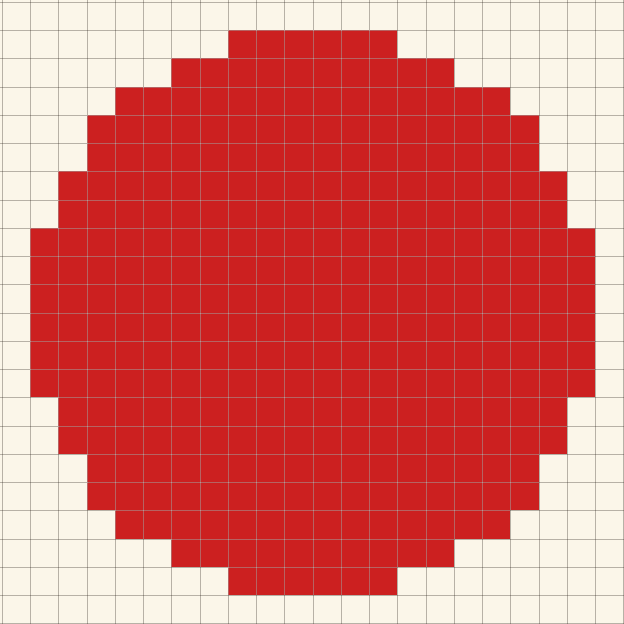
\includegraphics[width=\linewidth]{fig01_2d_d20_euclidean.png}
  \caption{\emph{Euclidean}}
\end{subfigure}\hfill
\begin{subfigure}[t]{0.31\linewidth}\centering
  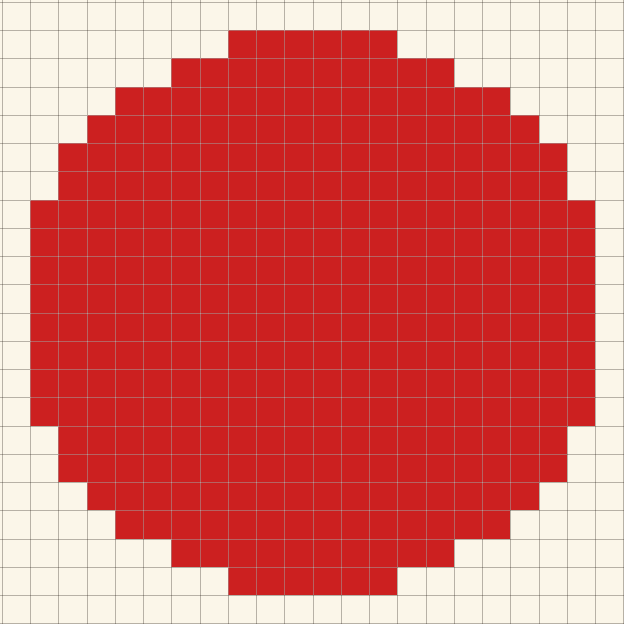
\includegraphics[width=\linewidth]{fig02_2d_d20_bresenham.png}
  \caption{\emph{Bresenham}}
\end{subfigure}\hfill
\begin{subfigure}[t]{0.31\linewidth}\centering
  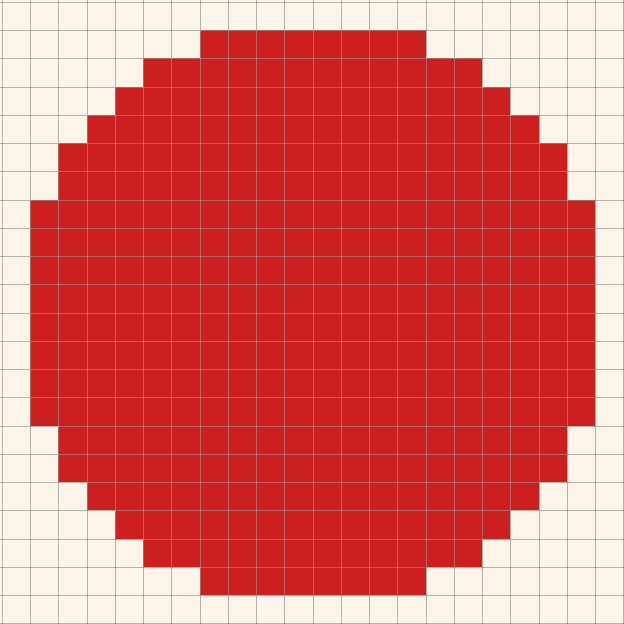
\includegraphics[width=\linewidth]{fig03_2d_d20_threshold.png}
  \caption{\emph{Threshold}}
\end{subfigure}
\caption{Same diameter-20 circle across the three algorithms. With larger diameters, differences are subtler than at small diameters.}
\label{fig:comp-d20}
\end{figure}


% =============================================================================
\subsection{Lesson 3 --- ``Into the third dimension: spheres, ellipsoids, slices''}

\subsubsection*{Lesson objective}
Generalize the ellipse equation to the ellipsoid; introduce voxels and discrete volume; understand planar cuts.

\begin{activity}[3.1 --- Engage: the 3D leap \quad\timing{15 min}]
Add a third coordinate $z$ to the plane. The ellipse equation generalizes immediately:

\begin{formula}
\centering
$\displaystyle \left(\dfrac{x}{r_x}\right)^{\!2} + \left(\dfrac{y}{r_y}\right)^{\!2} + \left(\dfrac{z}{r_z}\right)^{\!2} \;=\; 1$
\end{formula}

When $r_x = r_y = r_z$, it becomes the \acc{sphere} $x^2 + y^2 + z^2 = r^2$.

\textbf{Vocabulary anchor.} A 3D cell is called a \emph{voxel} (\emph{volume element}). The membership rule is identical to 2D but with three coordinates:

\begin{formula}
\centering
$\displaystyle a_x^2 + a_y^2 + a_z^2 \leq 1,\quad a_\xi = \dfrac{\xi + \tfrac{1}{2} - c_\xi}{r_\xi}$
\end{formula}

\textbf{Live demo.} Switch Pixel Round to 3D, then Ellipsoid. Drag to orbit. Switch the 3D render style (Classic / Smooth / Blocks). Toggle the edge overlay (the Grid button in 3D). Project as fullscreen.
\end{activity}
\begin{figure}[H]
\centering
\begin{subfigure}[t]{0.42\linewidth}\centering
  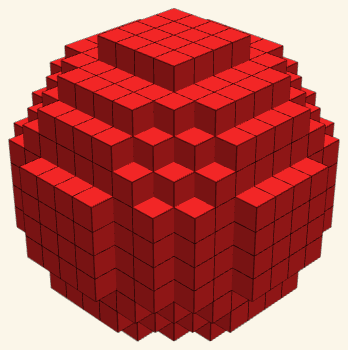
\includegraphics[width=\linewidth]{fig07_3d_sphere_d12.png}
  \caption{Sphere $D = 12$ ($r_x = r_y = r_z = 6$).}
\end{subfigure}\hfill
\begin{subfigure}[t]{0.42\linewidth}\centering
  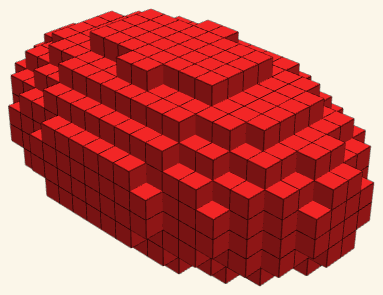
\includegraphics[width=\linewidth]{fig08_3d_ellipsoid.png}
  \caption{Ellipsoid $W = 20, H = 10, D = 12$.}
\end{subfigure}
\caption{3D voxelisation. Each cube is a voxel whose center coordinate is tested against the implicit equation.}
\label{fig:3d-shapes}
\end{figure}


\begin{activity}[3.2 --- Explain \& Elaborate: continuous vs.\ discrete volume \quad\timing{15 min}]
Continuous volume of an ellipsoid (a classic calculus result):

\begin{formula}
\centering
$\displaystyle V \;=\; \dfrac{4}{3}\,\pi\, r_x\, r_y\, r_z$
\end{formula}

When $r_x = r_y = r_z = r$, $V = \tfrac{4}{3}\pi r^3$. This formula appears regularly on the AP Calculus exam (free-response volume problems) and on standardized state assessments.

\textbf{Pair task:}
\begin{enumerate}[leftmargin=1.5em,itemsep=0.15em,topsep=0.3em,nosep]
  \item Compute the continuous volume of a sphere with diameter 12 ($r = 6$): $V = \tfrac{4}{3}\pi \cdot 216 \approx 904.78$.
  \item In Pixel Round, generate a sphere with diameter 12, Filled mode. Read the discrete volume.
  \item Compute the percent error.
\end{enumerate}

\textbf{Discussion.} The discrete-to-continuous ratio approaches 1 as $D \to \infty$ but diverges noticeably for small $D$ --- and that's mathematically correct: the discretization itself changes the count.
\end{activity}

\begin{activity}[3.3 --- Cuts as linear inequalities \quad\timing{10 min}]
Pixel Round offers three cut planes. Each is a \acc{linear inequality} applied to the voxel's center:

\begin{formula}
\centering
$\begin{array}{lcl}
\text{X cut:} & x \geq \mathit{cut} & \Rightarrow \text{voxel discarded} \\
\text{Y cut:} & y \geq \mathit{cut} & \Rightarrow \text{voxel discarded} \\
\text{Diagonal:} & x + y \geq \mathit{cut} & \Rightarrow \text{voxel discarded}
\end{array}$
\end{formula}

\textbf{Demo.} Cut a sphere by Y at 50\%. Then switch to the diagonal at 50\%. \emph{``Why does the diagonal slider run from 0 to $D_x + D_y$ and not just $D_x$? Where in this equation is the answer?''}
\end{activity}
\begin{figure}[H]
\centering
\begin{subfigure}[t]{0.31\linewidth}\centering
  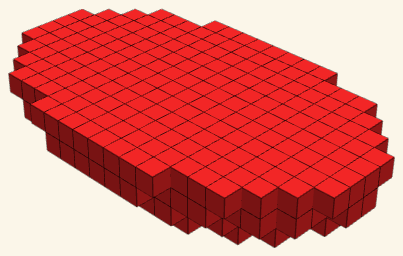
\includegraphics[width=\linewidth]{fig09_3d_cut_y50.png}
  \caption{Cut Y at 50\% ($y \geq 5$ discarded)}
\end{subfigure}\hfill
\begin{subfigure}[t]{0.31\linewidth}\centering
  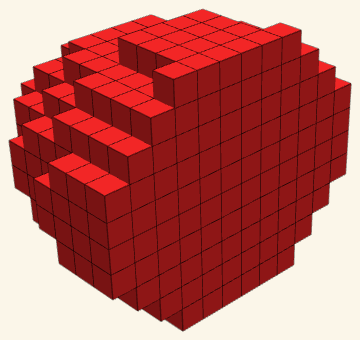
\includegraphics[width=\linewidth]{fig10_3d_cut_x50.png}
  \caption{Cut X at 50\% ($x \geq 10$ discarded)}
\end{subfigure}\hfill
\begin{subfigure}[t]{0.31\linewidth}\centering
  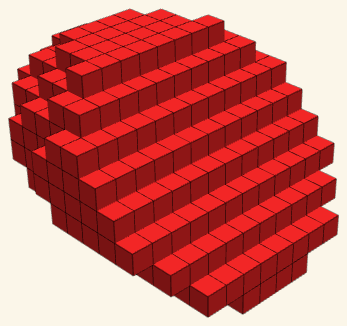
\includegraphics[width=\linewidth]{fig11_3d_cut_diag50.png}
  \caption{Diagonal cut ($x + y \geq 15$ discarded)}
\end{subfigure}
\caption{Three planar cuts on the same ellipsoid ($W = 20, H = 10, D = 12$), each preserving 50\% of the volume. Note the staircase pattern of the diagonal cut.}
\label{fig:cortes}
\end{figure}


\begin{activity}[3.4 --- Real-world connection: Minecraft \quad\timing{10 min}]
Show a few screenshots of Minecraft spheres built by players. Project Block Round (the companion project; same algorithms, block textures).

\textbf{Open discussion.} \emph{``You all have made a Minecraft sphere. Was it easy? Why or why not? Which of our three algorithms would you want as a Minecraft mod?''}

This is a deliberate hook into student culture: math becomes the language for explaining something they already do.
\end{activity}

% =============================================================================
\subsection{Lesson 4 --- ``Final project: original pixel art with a math defense''}

\subsubsection*{Lesson objective}
Synthesize the unit in an original product; assess via a defense in mathematical language.

\begin{activity}[4.1 --- Engage: the challenge \quad\timing{5 min}]
\textbf{Prompt:} \emph{``In pairs or triads, produce a pixel-art or voxel-art image that combines at least three figures generated by Pixel Round (circles, ellipses, spheres, ellipsoids). It can be a character, an icon, a logo --- you decide. At the end, your group will present and defend the work mathematically: why this algorithm? why this proportion? why this cut?''}

\textbf{Grouping.} Pre-assigned, mixed-readiness triads. 1 minute to take seats.
\end{activity}

\begin{activity}[4.2 --- Elaborate: production \quad\timing{30 min}]
\textbf{Per-group materials:}
\begin{itemize}[leftmargin=1.3em,itemsep=0.15em,topsep=0.3em,nosep]
  \item Chromebook or shared device with Pixel Round;
  \item Graph paper, pencils, colored markers for sketching;
  \item Roteiro handout (Appendix~\ref{ap:hw}, Exercise~5) with three required questions.
\end{itemize}

\textbf{Internal phases:}
\begin{enumerate}[leftmargin=1.5em,itemsep=0.15em,topsep=0.3em,nosep]
  \item \timing{5 min} brainstorm; rough sketch on paper.
  \item \timing{15 min} produce in Pixel Round; export each piece as PNG.
  \item \timing{5 min} assemble (re-trace onto graph paper with colored markers, or compose in slides/PowerPoint).
  \item \timing{5 min} write the mathematical defense on the handout.
\end{enumerate}

\textbf{Teacher role.} Circulate. Ask probing questions: \emph{``Why this algorithm? How would you describe that cut as an inequality? Could you build this in Minecraft with the same parameters?''}
\end{activity}

\begin{activity}[4.3 --- Evaluate: presentations and synthesis \quad\timing{15 min}]
Each group has 2 minutes to present, showing the work and answering at least one of three required questions.

\textbf{Minimum presentation criteria:}
\begin{itemize}[leftmargin=1.3em,itemsep=0.1em,topsep=0.2em,nosep]
  \item identify at least one mathematical figure in the work;
  \item name the chosen algorithm and justify (even \emph{post-hoc}) why it fits;
  \item if there's a 3D cut, describe it as an inequality.
\end{itemize}

\textbf{Closing synthesis (teacher, 3 min):} return to the unit's enduring understanding --- \emph{``on a discrete grid, the same continuous curve admits multiple representations; choosing one is a mathematical decision.''} Announce summative deadlines.
\end{activity}

% =============================================================================
\section{Assessment}

The plan uses three layers of assessment in line with backward design (Wiggins \& McTighe, 2005).

\subsection{Diagnostic}
During Lesson~1 Activity~1.2. The teacher walks the room and notes which students struggle with the coordinate plane, plotting, or rough sense of circle/diameter. Plan responsive scaffolds for Lesson~2.

\subsection{Formative}
Distributed: the Activity~1.4 exit ticket; the Activity~2.2 you-do; the percent error calculation in 2.5; the Activity~3.2 paired computation. Quick teacher feedback in the same period.

\subsection{Summative}
Two deliverables:

\begin{enumerate}[leftmargin=1.5em,itemsep=0.2em,topsep=0.3em,nosep]
  \item \textbf{Worksheet} (Appendix~\ref{ap:hw}), 5 problems, due at the end of Lesson 4 or as homework after.
  \item \textbf{Final project} (Activity~4.2), with the written defense.
\end{enumerate}

\subsection{Rubric}

\begin{center}
\small
\begin{tabularx}{\textwidth}{@{}p{0.20\textwidth}XX@{}}
\toprule
\textbf{Dimension} & \textbf{Proficient (3) / Advanced (4)} & \textbf{Developing (2) / Beginning (1)} \\
\midrule
\textbf{Mathematical concepts} & Applies the ellipse / ellipsoid equation correctly; distinguishes the three algorithms and predicts their differences. & Applies the basic circle equation but stumbles on the ellipse generalization, or confuses the three algorithms. \\
\addlinespace[3pt]
\textbf{Tool fluency} & Operates Pixel Round in 2D and 3D independently, exports PNGs, switches algorithms confidently. & Needs frequent assistance, operates only 2D. \\
\addlinespace[3pt]
\textbf{Argumentation} & Defends choices in the final project using precise math vocabulary (algorithm, voxel, cut, inequality, percent error). & Justifies aesthetically only; little math vocabulary in evidence. \\
\addlinespace[3pt]
\textbf{Collaboration} & Contributes productively to pair/triad work; participates in class discussion. & Works in isolation; minimal contribution. \\
\bottomrule
\end{tabularx}
\end{center}

\subsection{Grade weighting (suggested)}
\begin{itemize}[leftmargin=1.3em,itemsep=0.1em,topsep=0.2em,nosep]
  \item Worksheet: 40\%.
  \item Final project + defense: 50\%.
  \item Process observation (participation, group work): 10\%.
\end{itemize}

% =============================================================================
\section{Cross-curricular and out-of-classroom connections}

\subsection{Visual Art (digital media)}
The aesthetic of pixel art is widely treated as a visual-arts subject. Pixel Round is a rare opportunity to converge math and art on the same artifact: a figure is \emph{both} an equation and a composition. Suggested co-teach: an art department exhibition of student work in the hallway or on the school's Instagram.

\subsection{Physics (waves and acoustics)}
The Pixel Round sound layer uses additive synthesis of pure sine waves. The chosen frequencies approximate notes in the \acc{12-tone equal temperament} (each semitone multiplies frequency by $2^{1/12} \approx 1.0595$). Articulates with the AP Physics 1 wave unit and any treatment of musical acoustics.

\subsection{Computer Science (AP CSP, AP CSA)}
Bresenham's algorithm is a canonical undergraduate CS reference. The three Pixel Round algorithms are excellent case studies in computational thinking pillars: \emph{abstraction} (the equation as model), \emph{decomposition} (a shape as a union of cells), \emph{pattern recognition} (the eightfold symmetry), \emph{algorithm design} (three competing approaches). AP CSP teachers can use Activity~2.3 verbatim.

\subsection{College and career readiness}
The unit aligns naturally with the \acc{College Board's} list of skills appearing on the SAT (geometry of circles) and the AP Calculus AB free-response prompts on volumes of revolution. For students considering computer science, game design, or visual-effects careers, the unit is a glimpse of foundational professional skills.

% =============================================================================
\section{References}

\begin{itemize}[leftmargin=1.3em,itemsep=0.2em,topsep=0.3em]
  \item ANDERSON, L. W.; KRATHWOHL, D. R. (Eds.). \emph{A taxonomy for learning, teaching, and assessing: A revision of Bloom's taxonomy}. New York: Longman, 2001.
  \item BRESENHAM, J. E. Algorithm for computer control of a digital plotter. \emph{IBM Systems Journal}, v. 4, n. 1, p.~25--30, 1965.
  \item BYBEE, R. W. et al. \emph{The BSCS 5E Instructional Model: Origins and Effectiveness}. Colorado Springs: BSCS, 2006.
  \item CAST. \emph{Universal Design for Learning Guidelines version 2.2}. Wakefield, MA, 2018. Available at \texttt{udlguidelines.cast.org}.
  \item COMMON CORE STATE STANDARDS INITIATIVE. \emph{Common Core State Standards for Mathematics}. Washington, DC: NGA Center / CCSSO, 2010.
  \item NATIONAL COUNCIL OF TEACHERS OF MATHEMATICS. \emph{Principles to Actions: Ensuring Mathematical Success for All}. Reston, VA: NCTM, 2014.
  \item PITTEWAY, M. L. V. Algorithm for drawing ellipses or hyperbolae with a digital plotter. \emph{The Computer Journal}, v. 10, n. 3, p.~282--289, 1967.
  \item STIGLER, J. W.; HIEBERT, J. \emph{The Teaching Gap}. New York: Free Press, 1999.
  \item WIGGINS, G.; McTIGHE, J. \emph{Understanding by Design}. 2nd ed. Alexandria, VA: ASCD, 2005.
  \item Pixel Round technical companion: \texttt{docs\_math/Pixel\_Round\_Math\_en-US.pdf}.
\end{itemize}

\newpage
% =============================================================================
% APPENDICES
% =============================================================================
\appendix
\renewcommand{\thesection}{\Alph{section}}
\setcounter{section}{0}

\section{Live-demonstration script for Pixel Round}\label{ap:script}

Recommended sequence for the Lesson~1 demonstration and for first-time teacher familiarization. Total time: 15 minutes.

\subsection{Opening and 2D mode}
\begin{enumerate}[leftmargin=1.5em,itemsep=0.15em,topsep=0.3em]
  \item Open Pixel Round. Identify the topbar (mode + shape toggles), the canvas (center), and the controls (right panel on desktop, below the canvas on mobile).
  \item Confirm: \acc{2D / Circle}.
  \item Set Size slider to 10. Observe the figure.
  \item Click the Info chip in the canvas corner. Read aloud: ``Diameter 10, Radius 5, Area $\dots$, Algorithm Euclidean.''
  \item Toggle the algorithm pills: \acc{Euclidean / Bresenham / Threshold}. Pause 30 seconds on each.
\end{enumerate}

\subsection{Ellipse}
\begin{enumerate}[leftmargin=1.5em,itemsep=0.15em,topsep=0.3em]
  \item Switch to \acc{Ellipse}. The Size slider is replaced by Width + Height.
  \item Set $W = 16$, $H = 8$.
  \item Discussion: \emph{``The equation here is $(x/8)^2 + (y/4)^2 = 1$. Why divide $x$ by 8 and $y$ by 4?''}
\end{enumerate}

\subsection{3D mode}
\begin{enumerate}[leftmargin=1.5em,itemsep=0.15em,topsep=0.3em]
  \item Switch to \acc{3D / Sphere}, $D = 12$.
  \item Drag with mouse to rotate. A voxel sphere appears.
  \item Read the Info chip: record the volume.
  \item Switch to \acc{Ellipsoid}: $W = 20, H = 10, D = 10$.
  \item Demonstrate the \acc{Cut slider} on the Y axis at 50\%. The top half disappears.
  \item Switch to the diagonal axis ($\swarrow$ / $\nearrow$). Discuss the oblique cut.
\end{enumerate}

\subsection{Export}
\begin{enumerate}[leftmargin=1.5em,itemsep=0.15em,topsep=0.3em]
  \item Use the Download button in the canvas corner.
  \item Save the PNG to the device's Downloads folder.
  \item Note: the PNG comes out at high resolution --- suitable for printing, projecting, or embedding in a multimedia essay.
\end{enumerate}

% =============================================================================
\newpage
\section{Student worksheet}\label{ap:hw}

\textbf{Instructions.} Answer individually. You may verify answers in Pixel Round, but the \emph{mathematical justification is required}. Hand-written or typed. Due Lesson 4 (or per teacher).

\subsection*{Problem 1 --- Equation of a circle}
A circle is centered at the origin $(0, 0)$ with radius $r = 7$. For each point below, decide if it is \emph{inside}, \emph{outside}, or \emph{on} the circle. Justify with the inequality.
\begin{enumerate}[label=\alph*),leftmargin=1.5em,itemsep=0.1em,topsep=0.2em,nosep]
  \item $(3, 4)$ \hfill \emph{key:} inside ($9 + 16 = 25 < 49$).
  \item $(5, 5)$ \hfill \emph{key:} outside! ($25 + 25 = 50 > 49$, since $\sqrt{50} \approx 7.07$).
  \item $(0, 7)$ \hfill \emph{key:} on.
  \item $(-7, 0)$ \hfill \emph{key:} on.
\end{enumerate}

\subsection*{Problem 2 --- Euclidean rule applied to one cell}
A circle is centered at $(5, 5)$ with radius $5$. Apply the Euclidean rule to cell $(i, j) = (1, 3)$: is it filled?

\emph{Key:} cell center $(1.5,\, 3.5)$. Distance to $(5, 5)$: $\sqrt{(5-1.5)^2 + (5-3.5)^2} = \sqrt{12.25 + 2.25} = \sqrt{14.5} \approx 3.81 < 5$. \acc{Filled}.

\subsection*{Problem 3 --- Discrete area vs.\ continuous area}
In Pixel Round, generate a Euclidean circle with diameter 20. Read the discrete area (Info chip). Compute the continuous area $\pi r^2$. Compute the percent error. Repeat for the Threshold algorithm. Compare.

\emph{Key:} continuous area $= 100\pi \approx 314.16$. Euclidean typically within 2\%. Threshold overshoots by 5--8\%.

\subsection*{Problem 4 --- Volume of an ellipsoid and a cut}
An ellipsoid has semi-axes $r_x = 4$, $r_y = 6$, $r_z = 3$.
\begin{enumerate}[label=\alph*),leftmargin=1.5em,itemsep=0.1em,topsep=0.2em,nosep]
  \item Compute the continuous volume.
  \item After a Y-axis cut that preserves $50\%$ of the height, what is the remaining volume (continuously)?
  \item Describe the cut as an inequality on the voxel's $y$-coordinate.
\end{enumerate}

\emph{Key:} (a) $V = \tfrac{4}{3}\pi \cdot 4 \cdot 6 \cdot 3 = 96\pi \approx 301.59$.
(b) By symmetry, $\approx 150.80$.
(c) $y < \mathit{cut}$, where $\mathit{cut} = 0.5 \cdot D_y = 0.5 \cdot 12 = 6$.

\subsection*{Problem 5 --- Final-project written defense}
After producing the original work in your group (Activity~4.2), answer in writing:
\begin{enumerate}[label=(\arabic*),leftmargin=1.7em,itemsep=0.15em,topsep=0.2em,nosep]
  \item List the geometric figures used (circle, ellipse, sphere, ellipsoid) with their parameters (diameter or semi-axes).
  \item For the main figure, which algorithm did you choose, and why? What visual effect does it produce that the other two would not?
  \item Did you use any 3D cuts? If so, describe \emph{one} of them as an inequality.
\end{enumerate}

% =============================================================================
\newpage
\section{Adaptation for low-resource classrooms}\label{ap:adapt}

This adaptation supports running the full sequence \emph{entirely on paper} when one-to-one device access is unavailable. The conceptual core is preserved; only the medium changes.

\subsection{Substitutions by lesson}

\begin{center}
\small
\begin{tabularx}{\textwidth}{@{}p{0.16\textwidth}p{0.36\textwidth}X@{}}
\toprule
\textbf{Lesson} & \textbf{Original activity} & \textbf{Analog substitute} \\
\midrule
1 & Pixel Round demo (1.3) & Teacher draws the three rule-circles by hand on a board-sized grid (pre-drawn with grid lines), one per algorithm. \\
\addlinespace[3pt]
2 & Software comparison (2.5) & Distribute pre-printed handouts showing the three diameter-16 circles. Students count cells manually. \\
\addlinespace[3pt]
3 & 3D sphere generation (3.1, 3.2) & Distribute pre-printed sheets with the \emph{slices} of the sphere ($z = 0, 1, 2, \ldots$) on graph paper. Students mentally stack them. \\
\addlinespace[3pt]
4 & Pixel Round production (4.2) & Production \emph{exclusively} on graph paper with colored pencils. The math defense (4.3) is unchanged. \\
\bottomrule
\end{tabularx}
\end{center}

\subsection{Preparation kit (one-time)}
\begin{itemize}[leftmargin=1.3em,itemsep=0.1em,topsep=0.2em,nosep]
  \item One 17$\times$22 in.\ poster with a $30 \times 30$ grid (use chart paper or a vinyl battle map).
  \item One classroom set (30) of graph-paper packets (4 sheets each).
  \item One pre-printed reference sheet showing the three comparison circles (generate in Pixel Round at home, export, print).
\end{itemize}

\subsection{State variations crosswalk}\label{ap:adapt-states}

For schools in non-CCSS states, the following crosswalk maps the lesson to local standards:

\begin{center}
\small
\begin{tabularx}{\textwidth}{@{}p{0.14\textwidth}p{0.20\textwidth}X@{}}
\toprule
\textbf{State} & \textbf{Standard set} & \textbf{Closest matching standards} \\
\midrule
Texas & TEKS (Geometry) & G.12.A (circle equations), G.12.D--E (volume \& cross-sections), G.13 (probability/area applications). \\
\addlinespace[3pt]
Virginia & Mathematics SOL & G.10 (volume \& surface area), G.11 (similar/congruent figures in coordinate plane). \\
\addlinespace[3pt]
Florida & B.E.S.T.\ Standards & MA.912.GR.6 (circle equations), MA.912.GR.7 (volume/surface area). \\
\bottomrule
\end{tabularx}
\end{center}

\textit{Note.} The activities themselves require no modification; only the alignment table on the cover page should be replaced for documentation purposes (administrator audits, portfolio submissions).

% =============================================================================
\newpage
\section{Teacher's technical glossary}\label{ap:glossary}

\begin{itemize}[leftmargin=1.4em,itemsep=0.3em,topsep=0.3em]
  \item \acc{Algorithm} --- a finite, well-defined sequence of instructions for solving a problem. The three Pixel Round algorithms are distinct procedures for the same problem (deciding which cells to fill).
  \item \acc{Bresenham (algorithm)} --- the 1965 algorithm by Jack Bresenham of IBM, originally for lines, later extended to circles and (by Pitteway and Kappel) to ellipses. Its signature trait: integer-only arithmetic.
  \item \acc{Canvas} --- HTML element providing a 2D or 3D drawing surface in the browser, pixel-by-pixel or via WebGL.
  \item \acc{Implicit equation} --- an equation of the form $F(x, y) = 0$, defining a curve as the \emph{zero set} of a function, rather than $y = f(x)$ (explicit form). For the ellipse: $(x/r_x)^2 + (y/r_y)^2 - 1 = 0$.
  \item \acc{PWA --- Progressive Web App} --- a web app installable on a device and operable offline. Pixel Round is a PWA: a single visit on Wi-Fi caches the entire app.
  \item \acc{Pixel} --- short for \emph{picture element}. Minimum unit of a digital image; in a grid, occupies a $1 \times 1$ cell.
  \item \acc{Rasterization} --- conversion of a continuous geometric description into a grid of pixels (2D) or voxels (3D).
  \item \acc{Semi-axis} --- in an ellipse centered at $C$, the distance from $C$ to the ellipse along the named axis. The circle is the special case with $r_x = r_y = r$.
  \item \acc{12-tone equal temperament} --- division of the octave into 12 equal intervals (semitones). The frequency ratio between consecutive semitones is $\sqrt[12]{2} \approx 1.0595$. Foundation of Western music.
  \item \acc{Voxel} --- short for \emph{volume element}. The 3D generalization of a pixel: a $1 \times 1 \times 1$ cubic cell in a 3D grid.
  \item \acc{WebGL} --- low-level 3D graphics API for browsers. Pixel Round uses it (through three.js) to render the 3D scene.
\end{itemize}

\vspace{2em}
\begin{center}
\color{muted}\small\sffamily
--- end of lesson plan ---
\end{center}

\end{document}
